\chapter{Основные понятия и определения теории каскадов}\label{ch2_theory}

Наряду с развитием технологий разделения изотопов развивается также и теория каскадов для разделения изотопных смесей. За последние десятилетия в ней достигнуты значительные успехи в части описания процессов молекулярно-селективного массопереноса при разделении многокомпонентных смесей физическими методами. Весомый вклад в развитие теории внесли научные группы УрФУ им. Б.Н. Ельцина (В.А. Палкин и др.), НИУ ТПУ (А.А. Орлов и др.), НИЯУ МИФИ (Г.А. Сулаберидзе, А.Ю. Смирнов, В.Д. Борисевич), университета Цинхуа (г. Пекин, КНР), а также коллективы расчетных групп на разделительных производствах (АО <<СХК>>, АО <<ПО ЭХЗ>>, АО <<УЭХК>> и др.). Предложенные модели могут быть использованы, в том числе, для изучения физических закономерностей процесса обогащения регенерированного урана, который, в отличие от природного урана, нельзя упрощенно рассматривать в качестве бинарной смеси.
Ниже, кратко приведены основные понятия из теории каскадов для разделения многокомпонентных смесей, а также использованные в рамках данной работы модели каскадов для разделения многокомпонентных смесей.

\section{Основы теории разделения в каскадах}

% На сегодняшний день разработан обширный набор расчетных моделей, которые могут быть применены в том числе и к задаче обогащения регенерированного урана \cite{smirnovMolekulyarnoselektivnyyMassoperenosKomponentov2013}. Введем основные теоретические понятия и рассмотрим модельные каскады, релевантные задаче  работы.

\subsection{Понятие разделительной ступени}

Рассмотрим общие характеристики разделительных ступеней, предназначенных для разделения многокомпонентных изотопных смесей в газовой фазе. В качестве разделяемой изотопной смеси рассмотрена смесь, содержащая \textit{m} химически не реагирующих между собой компонентов, содержание можно определять либо мольно-долевыми концентрациями, либо массовыми $C_{i}$ ($i=1,...,m$) \cite{sulaberidzeTeoriyaKaskadovDlya2011}. Компоненты пронумерованы в порядке возрастания массовых чисел изотопов урана в смеси. В рамках настоящего исследования будут использованы массовые концентрации. С учетом этого, в случае разделения смесей изотопов тяжелых химических элементов, включая уран, численные значения массовых и мольных долей приблизительно совпадают \cite{sulaberidzeTeoriyaKaskadovDlya2011}.  Для концентраций компонентов разделяемой смеси справедливо очевидное тождество:

\begin{equation} \label{GrindEQ__1_1_} 
  \sum _{j=1}^{m}C_{j}  =1 
\end{equation} 
  
Наряду с абсолютными концентрациями $C_{i} $ часто используют относительные концентрации, определяемые по отношению к концентрации так называемого «опорного» компонента с фиксированным номером, например, \textit{k}, то есть

\begin{equation} \label{GrindEQ__1_2_} 
  R_{ik} =\frac{C_{i} }{C_{k} } ,\;\;  i=1,...,m.             
\end{equation} 
  
В качестве <<опорного>> может быть выбран любой из компонентов смеси. 
Простая трехпоточная разделительная ступень имеет один входной поток и два выходных (рисунок \ref{1_1}). На вход ступени поступает поток питания (производительность ступени) $L$  (в системе СИ в кг/с) с концентрациями $C_{i}$ ($i=1,...,m$). Из ступени выходят два потока: легкая фракция (поток, обогащенный легкими компонентами) или отбор ступени $L'$ и тяжелая фракция (поток, обедненный легкими компонентами) или отвал ступени $L''$. Концентрации компонентов в этих потоках  $C'_{i} $ и $C''_{i} $, соответственно.

\begin{figure}[ht]
  \centerfloat{\includegraphics[scale=0.3]{images/theory/sep_el_n}}
  \caption{Схема трехпоточной разделительной ступени}\label{1_1}
\end{figure}

Коэффициент деления потока смеси (срез) $\theta$, парциальные потоки компонентов $L_{i} ,\; L'_{i} ,\; L''_{i}$ и срезы парциальных потоков $\phi _{i}$ можно определить по формулам:

\begin{equation} \label{GrindEQ__1_3_} 
  \theta =\frac{L'}{L} ,\;\;  L_{i} =L \cdot C_{i} ,\;\;  L'_{i} =L' \cdot C'_{i} ,\;\;  L''_{i} =L'' \cdot C''_{i} , 
  \end{equation} 
  \begin{equation} \label{GrindEQ__1_4_} 
  \phi _{i} =\frac{L'_{i} }{L_{i} } ,\;\;  1-\phi _{i} =\frac{L''_{i} }{L_{i} } ,\;\; i=1,...,m. 
  \end{equation} 

В стационарном режиме работы и в отсутствие потерь рабочего вещества потоки ступени связаны уравнениями баланса:

\begin{equation} \label{GrindEQ__1_5_} 
  L=L'+L'', 
  \end{equation} 
  \begin{equation} \label{GrindEQ__1_6_} 
  L_{i} =L'_{i} + L''_{i} ,\;\; i=1,...,m.             
\end{equation} 
  
Введенное в \ref{GrindEQ__1_3_} определение среза потоков ступени дает возможность представить уравнения \ref{GrindEQ__1_6_} в следующем виде:

\begin{equation} \label{GrindEQ__1_7_} 
  C_{i} =\theta  \cdot C'_{i} +(1-\theta ) \cdot C''_{i} . 
\end{equation} 

Для каждого компонента $i$ с относительной концентрацией вводят относительные коэффициенты разделения: полный $q_{ik}$, в отборе (потоке легкой фракции) $\alpha _{ik} $ и в отвале (потоке тяжелой фракции) $\beta _{ik} $ и соответствующие коэффициенты обогащения $\varepsilon _{ik} ,\; \varepsilon '_{ik} ,\; \varepsilon ''_{ik} \; $
% \[q_{ik} =\frac{R'_{ik} }{R''_{ik} } ,\; \; \alpha _{ik} =\frac{R'_{ik} }{R_{ik} } ,\; \; \beta _{ik} =\frac{R_{ik} }{R''_{ik} } ,\] 

\begin{equation} \label{GrindEQ__1_11_} 
  \begin{array}{l}
    \qquad q_{i k}=\frac{R_{i k}^{\prime}}{R_{i k}^{\prime \prime}},\;\; \alpha_{i k}=\frac{R_{i k}^{\prime}}{R_{i k}},\;\; \beta_{i k}=\frac{R_{i k}}{R_{i k}^{\prime \prime}} ;\;\; \\
    \varepsilon_{i k}=q_{i k}-1,\;\; \varepsilon_{i k}^{\prime}=\alpha_{i k}-1,\;\; \varepsilon_{i k}^{\prime \prime}=1-\frac{1}{\beta_{i k}} .
    \end{array}
\end{equation} 

При разделении изотопов молекулярно-кинетическими методами, включая метод газовой центрифуги, величины полных относительных коэффициентов разделения можно аппроксимировать соотношениями $q_{ij} =q_{0} {}^{M_{j} -M_{i} }$, где $q_0$ --- коэффициент разделения, приходящийся на единицу разности массовых чисел; \textit{M${}_{i}$, M${}_{j}$} --- массовые числа $i$-го и $j$-го компонентов, соответственно \cite{sulaberidzeTeoriyaKaskadovDlya2011}.

Если $k\ne m$, то при всех $i<k$ значения всех коэффициентов разделения $q_{ik}$, $\alpha _{ik}$, $\beta _{ik}$, будут больше единицы, а при всех $i>k$ --- меньше единицы.

Полные коэффициенты разделения $q_{ik} $, как правило, не зависят от состава смеси. В некоторых случаях, что характерно для газовой центрифуги, коэффициенты $q_{ik}$ могут зависеть от коэффициента деления потока $\theta$ и от потока питания $L$ (\ref{GrindEQ__q_}) единичного разделительного элемента (ступени) \cite{mustafinObjectiveFunctionOptimization2019}:

\begin{equation} \label{GrindEQ__q_} 
  q_{ij} = f(\theta, L)          
\end{equation}

В практических расчетах при определении оптимальных параметров разделительного каскада необходимо учитывать конкретный вид зависимости (\ref{GrindEQ__q_}), которой может быть получен теоретически путем решения задачи конвективной диффузии для одиночного разделительного аппарата. После чего зависимость может быть уточнена на основе экспериментальных данных. 
Анализ зависимостей вида (\ref{GrindEQ__q_}) для различных газовых центрифуг показывает, что часть данной функции, определяемая величиной $\theta$ представляет собой гладкую функцию с одним экстремумом (максимумом). В теоретических исследованиях часто используют упрощенные подходы, в которых либо пренебрегают зависимостью коэффициентов разделения от какого-либо из указанных выше параметров, либо от всех, считая коэффициенты разделения одинаковыми на всех ступенях. Например, можно пренебречь зависимостью величины коэффициента разделения от $\theta$, осуществив предварительное усреднение функции (\ref{GrindEQ__q_}) по этому параметру и выбрав оптимальную с точки зрения разделительной способности элемента величину потока питания $L$. Такой подход как в случае разделения бинарных, так и многокомпонентных смесей приводит к теории так называемых «модельных каскадов» (каскадов с одинаковыми по ступеням коэффициентами разделения) \cite{24sulaberidzeClassificationModelCascades2020}.

Данный подход использован и в настоящем исследовании (каскады, состоящие из разделительных элементов, имеющих одинаковые коэффициенты разделения и работающих в идентичных режимах). Учет зависимости от $\theta$ ($g(\theta)$) может быть использован в <<уточняющих>> расчетах.

В дополнение к введенным выше параметрам также используют величины $g_{i}$, которые можно рассматривать как отношение парциальных потоков компонентов в легкой и тяжелой фракциях, покидающих ступень:

\begin{equation} \label{GrindEQ__1_13_} 
  g_{i} =\frac{\phi _{i} }{1-\phi _{i} } =\frac{L'_{i} }{L''_{i} } ,\; \; i\ne k, 
  \end{equation} 
  \begin{equation} \label{GrindEQ__1_14_} 
  g_{k} =\frac{\phi _{k} }{1-\phi _{k} } =\frac{L'_{k} }{L''_{k} } .           
\end{equation} 

Нетрудно показать, используя \ref{GrindEQ__1_11_}--\ref{GrindEQ__1_14_}, что величины $g_{i}$ и $g_{k}$, являющаяся инвариантом, связаны с величинами относительных коэффициентов разделения следующими соотношениями:

\begin{equation} \label{EQ__1_15_} 
  g_{i} =\frac{\alpha _{ik}  \cdot (\beta _{ik} -1)}{\alpha _{ik} -1} ,\; \; i\ne k,           
  \end{equation} 
  \begin{equation} \label{EQ__1_16_} 
  g_{k} =\frac{\beta _{ik} -1}{(\alpha _{ik} -1) \cdot \beta _{ik} } =\frac{\varepsilon ''_{ik} }{\varepsilon '_{ik} } . 
\end{equation} 

При этом

\begin{equation} \label{EQ__1_17_} 
  \frac{g_{i} }{g_{k} } =q_{ik} .           
\end{equation} 

С использованием выражений \ref{GrindEQ__1_1_}--\ref{EQ__1_17_} получим следующие соотношения, связывающие параметры отдельной ступени каскада:

\begin{equation} \label{GrindEQ__1_18_} 
  L=\sum _{j=1}^{m}L_{i}  =\sum _{j=1}^{m}\frac{g_{i} +1}{g_{i} } \cdot L_{i} ',               
  \end{equation} 
  \begin{equation} \label{GrindEQ__1_19_} 
  C_{i} =\frac{g_{i} +1}{g_{i} } \cdot \frac{L_{i} '}{L} ,         
\end{equation}   

\subsection{Симметричный противоточный каскад и система уравнений, описывающих для него массоперенос в общем виде}

Как известно, при практической реализации многих методов разделения используют многоступенчатые разделительные установки, называемые каскадами \cite{sulaberidzeTeoriyaKaskadovDlya2011}. Подобные установки представляют собой последовательно соединенные ступени, состоящие из параллельно соединенных разделительных элементов, в частности газовых центрифуг.

Существуют различные способы коммутации ступеней в разделительных каскадах. Наиболее известен так называемый способ симметричного соединения ступеней в противоточной схеме (рисунок \ref{1_2}), когда поперечное сечение, проведенное между любыми двумя ступенями каскада, будет пересекать две линии коммутации ступеней. Рассмотрим схему такого каскада, имеющего один входящий поток питания $F$ и два выходящих: отбор $P$, обогащенный самым легким компонентом и отвал $W$, обогащенный самым тяжелым компонентом. Потоки $F$, $P$, $W$ и концентрации компонентов в них $C_{i,F} ,\; \; C_{i,P} ,\; \; C_{i,W} \; \; (i=1,...,m)$ являются внешними параметрами каскада. Следует заметить, что в случае разделения многокомпонентных смесей понятия «отбор» и «отвал» условны, поскольку ценный компонент может обогащаться как вместе с самым легким компонентом смеси, так и вместе с самым тяжелым.

\begin{figure}[ht]
  \centerfloat{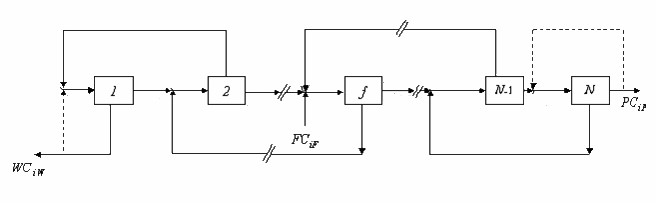
\includegraphics[scale=0.7]{images/theory/2}}
  \caption{Схема соединения ступеней в симметрично-противоточном каскаде}\label{1_2}
\end{figure}

В стационарном режиме работы и в отсутствии потерь рабочего вещества на ступенях каскада, внешние параметры каскада должны удовлетворять уравнениям материального баланса:

\begin{equation} \label{GrindEQ__1_21_} 
  \begin{array}{l} {\quad \quad \quad \quad F=P+W,} \\ {F \cdot C_{i,F} =P \cdot C_{i,P} +W \cdot C_{i,W} ,\; \; i=1,...,m.} \end{array} 
\end{equation} 

Ступени каскада пронумерованы последовательно от $s=1$ на отвальной ступени каскада до $s=N$ на отборной ступени. Считаем, что внешнее питание каскада ($F$) подают на вход ступени с номером $f$. Внутренние параметры произвольной ступени с номером \textit{s} ($L_{s} $, $L'_{s} ,$ $L''_{s} ,$ $L_{i,s} ,$ $L'_{i,s} ,$ $L''_{i,s} $), где $L$ --- потоки вещества, а $L_i$ --- парциальные потоки (изотопов с индексами $i$) в стационарном режиме работы каскада, в отсутствие потерь рабочего вещества на ступенях каскада связаны уравнениями \ref{GrindEQ__1_5_}-\ref{GrindEQ__1_6_}.

Уравнения баланса в «узлах» (точках соединения межступенных потоков) при симметричном соединении ступеней имеют вид:

\begin{subequations}\label{GrindEQ__1_24_}
  \begin{empheq}[left=\empheqlbrace]{align}
    &L_{s} =\theta _{s-1} \cdot L_{s-1} +(1-\theta _{s+1} ) \cdot L_{s+1} \, ,\; \; s=1,...,N   \\
    &L_{s} \cdot C_{i,s} =\theta _{s-1} \cdot L_{s-1} \cdot C'_{i,s-1} +(1-\theta _{s+1} ) \cdot L_{s+1} \cdot C''_{i,s+1} \, , \, s=1,...,N.
  \end{empheq}
\end{subequations}

Для ступени подачи питания $f$ аналогичные уравнения выглядят так:

\begin{subequations}\label{GrindEQ__1_27_}
  \begin{empheq}[left=\empheqlbrace]{align}
    &L_{f} =\theta _{f-1} \cdot L_{f-1} +(1-\theta _{f+1} ) \cdot L_{f+1} +F \\
    &L_{f} \cdot C_{i,f} =\theta _{f-1} \cdot L_{f-1} \cdot C'_{i,f-1} +(1-\theta _{f+1} ) \cdot L_{f+1}  \cdot C''_{i,f+1} + F \cdot C_{i,F} \, ,\quad i=1,...,m.
  \end{empheq}
\end{subequations}

Внешние и внутренние параметры каскада связаны граничными условиями:

\begin{equation} \label{GrindEQ__1_28_} 
  L_{0} =L'_{0} =L''_{0} =L_{N+1} =L'_{N+1} =L''_{N+1} =0, 
  \end{equation} 
  \begin{equation} \label{GrindEQ__1_29_} 
  L'_{N} =\theta _{N} \cdot L_{N} =P,        
  \end{equation} 
  \begin{equation} \label{GrindEQ__1_30_} 
  L''_{1} =(1-\theta _{1} )\cdot L_{1} =W,        
  \end{equation} 
  \begin{equation} \label{GrindEQ__1_31_} 
  C'_{N} =C_{i,P} \;, \; \;  i=1,...,m, 
  \end{equation} 
  \begin{equation} \label{GrindEQ__1_32_} 
  C''_{1} =C_{i,W} \;, \; \;  i=1,...,m, 
  \end{equation} 
  \begin{equation} \label{GrindEQ__1_33_} 
  L'_{i,N} =P \cdot C_{i,P} \; , \; \; i=1,...,m, 
  \end{equation} 
  \begin{equation} \label{GrindEQ__1_34_} 
  L''_{i,1} =W \cdot C_{i,W} \;, \; \; i=1,...,m. 
\end{equation} 

Соотношения (\ref{GrindEQ__1_21_})--(\ref{GrindEQ__1_34_}) описывают простейшую физико-математическую модель противоточного симметричного каскада, предназначенного для разделения многокомпонентной смеси. Анализ данной системы показывает, что она представляют собой системы нелинейных разностных уравнений относительно функций $C_{i,s}$. Существенной проблемой при решении подобных систем является то, что в эти уравнения (либо в их граничные условия) входят значения концентраций, которые неизвестны заранее и должны быть определены из решения этих же уравнений. В общем случае, система (\ref{GrindEQ__1_24_})--(\ref{GrindEQ__1_34_}) для своего решения требует использования численных методов.

Трудности решения (\ref{GrindEQ__1_24_})--(\ref{GrindEQ__1_34_}) в общем случае, стимулировали развитие упрощенных подходов, которые позволяют получить ее аналитическое решение при введении определенных предположений. Полученные в результате таких упрощений физико-математические модели симметрично-противоточного каскада сохраняют закономерности молекулярно-селективного массопереноса, но позволяют заметно упростить соответствующие расчетные процедуры для определения оптимальных параметров каскада. Такие каскады получили название модельных \cite{minenkoTeoriiKaskadovDlya1965, delagarzaMulticomponentIsotopeSeparation1961, zhigalovskiyLekcionnyeMaterialyPo1999, kolokoltsovDesignCascadesSeparating1970, 2024VoprosuPostroeniiKaskadov, minenkoPredelnoeObogashcheniePromezhutochnyh1972, yamamotoMulticomponentIsotopeSeparating1978, wuStudyMulticomponentIsotope, borisevichRascheteKaskadovDopolnitelnym1993, woodCriterionEffiencyMultiisotope1999, sulaberidzeOsobennostiObogashcheniyaKomponentov2006, sazykinKvaziidealnyeKaskadyDlya2000, sulaberidzeSravnenieOptimalnyhModelnyh2008}.

Как показали результаты теоретического анализа модельные каскады фактически представляют собой частный случай рассмотренного выше симметрично-противоточного каскада, отвечающий условию постоянства по его длине относительных коэффициентов разделения \cite{24sulaberidzeClassificationModelCascades2020}.  
Ниже кратко рассмотрены предложенные на текущий момент модельные каскады.

\subsection{«Квазиидеальный» каскад}

Рассмотрим случай симметричного противоточного каскада с постоянными по его длине относительными коэффициентами разделения $q_{ik} ,\; \alpha _{ik} ,\; \beta _{ik} $ $(i=1,...,m;$ \textit{k} --- номер «опорного» компонента). Это условие обеспечивает постоянство величин \textit{g${}_{i}$} и $\phi _{i} $. Следовательно, соотношения (\ref{GrindEQ__1_24_})--(\ref{GrindEQ__1_27_}) приводятся к виду \cite{sulaberidzeTeoriyaKaskadovDlya2011}:

\begin{equation} \label{GrindEQ__1_52_} 
  L'_{i} (s-1)+\frac{1}{g_{i}} \cdot L'_{i} (s+1)-\frac{g_{i} +1}{g_{i} }\cdot L'_{i} (s)+\delta _{sf} \cdot F \cdot C_{i,F} =0,\; \; i\ne k, 
  \end{equation} 
  \begin{equation} \label{GrindEQ__1_53_} 
  L'_{k} (s-1)+\frac{1}{g_{k}} \cdot L'_{k} (s+1)-\frac{g_{k} +1}{g_{k} }\cdot L'_{k} (s)+\delta _{sf} \cdot F \cdot C_{k,F} =0, 
\end{equation}
где $s$ – текущий номер ступени, отсчитываемый от «тяжелого» конца каскада к его «легкому» концу $\delta _{sf} =\left\{\begin{array}{l} {0,\; \; s\ne f} \\ {1,\; \; s=f} \end{array}\right.$

Уравнения (\ref{GrindEQ__1_52_})--(\ref{GrindEQ__1_53_}) представляют собой линейные разностные уравнения второго порядка относительно неизвестных функций $L'_{i} (s)$. Граничные условия для них имеют вид:

\begin{equation} \label{GrindEQ__1_54_} 
  \left\{\begin{array}{l} {L'_{i} (0)=L'_{i} (N+1)=0,\; \; i=1,...,m} \\
    {L'_{i} (N)=P \cdot C_{i,P} \; ,\; \; i=1,...,m} \\
    {L'_{i} (1)=g_{i} \cdot W \cdot C_{i,W} \; ,\; \; i\ne k} \\
    {L''_{k} (1)=g_{k} \cdot W \cdot C_{i,W} \; .} \end{array}\right.  
\end{equation} 

Решение системы уравнений (\ref{GrindEQ__1_52_})--(\ref{GrindEQ__1_53_}), с использованием уравнений баланса (\ref{GrindEQ__1_21_}) и граничных условий (\ref{GrindEQ__1_54_}), легко преобразуется в уравнения связи внешних параметров такого каскада с длинами его секций и параметрами ступени:

\begin{equation} \label{GrindEQ__1_55_} 
  \frac{P}{F} =\sum _{j=1}^{m}C_{j,F} \cdot \frac{1-g_{j}^{-f} }{1-g_{j}^{-N-1}} \; ,%\; \; s=f,...,N ,                                                  
  \end{equation} 
  \begin{equation} \label{GrindEQ__1_56_} 
  \frac{W}{F} =\sum _{j=1}^{m}C_{j,F} \cdot \frac{g_{j}^{N+1-f} -1}{g_{j}^{N+1} -1} \; ,%\; \; s=1,...,f-1 ,                                            
\end{equation}

\begin{equation} \label{GrindEQ__1_57_} 
  C_{i,P}=C_{i,F} \cdot \frac{1-g_{i}^{-f}}{1-g_{i}^{-N-1}} / \sum_{j=1}^{m} C_{j,F} \cdot \frac{1-g_{j}^{-f}}{1-g_{j}^{-N-1}}\; ,\; \;  i=1, \ldots, m                             
\end{equation}

\begin{equation} \label{GrindEQ__1_58_} 
  C_{i,W}=C_{i,F} \cdot \frac{g_{i}^{N+1-f}-1}{g_{i}^{N+1}-1} / \sum_{j=1}^{m} C_{j,F} \cdot \frac{g_{j}^{N+1-f}-1}{g_{j}^{N+1}-1}\; ,\; \;  i=1, \ldots, m                         
\end{equation} 

Далее, распределение потока $L(s)$, концентраций компонентов и коэффициента деления потока по ступеням каскада можно определить по формулам \cite{sulaberidzeTeoriyaKaskadovDlya2011}:

\begin{equation} \label{GrindEQ__1_59_} 
  L(s)=\sum_{j=1}^{m} L_{j}^{\prime}(s) \cdot \frac{1+g_{j}}{g_{j}}=\left\{\begin{array}{c}
  P \cdot \sum_{j=1}^{m} \frac{g_{j}+1}{g_{j}-1} \cdot C_{j,P} \cdot \left(1-g_{j}^{s-N-1}\right)  ,\; \;  s=f, \ldots, N \\
  W \cdot \sum_{j=1}^{m} \frac{g_{j}+1}{g_{j}-1} \cdot C_{j,P} \cdot \left(g_{j}^{s}-1\right) ,\; \;  s=1, \ldots, f-1,
  \end{array}\right.
\end{equation} 

\begin{equation} \label{GrindEQ__1_60_} 
  C_{i} (s)=\frac{1+g_{j} }{g_{j} } \cdot \frac{L''_{i} (s)}{L_{i} (s)} =\left\{\begin{array}{l} {\frac{C_{i,P}\cdot \frac{g_{j} }{g_{j} -1}\cdot \left(1-g_{j}^{s-N-1} \right)}{\sum _{j=1}^{m}\frac{g_{j} +1}{g_{j} -1} \cdot C_{j,P} \cdot \left(1-g_{j}^{s-N-1} \right)} \; ,\; \; s=f,...,N} \\ {\; \frac{C_{i,W} \cdot \frac{g_{j} }{g_{j} -1} \cdot \left(g_{j}^{s} -1\right)}{\sum _{j=1}^{m}\frac{g_{j} +1}{g_{j} -1} \cdot C_{j,W} \cdot \left(g_{j}^{s} -1\right)} \; ,\; \; s=1,...,f-1,} \end{array}\right.  
\end{equation} 

\begin{equation} \label{GrindEQ__1_61_} 
  \begin{array}{l} {\theta (s)=\frac{\sum _{j=1}^{m}L'_{j} (s) }{\sum _{j=1}^{m}L_{j} (s) } =\left\{\begin{array}{l} {\frac{\sum _{j=1}^{m}\frac{g_{j} }{g_{j} -1} \cdot C_{j,P} \cdot \left(1-g_{j}^{s-N-1} \right) }{\sum _{j=1}^{m}\frac{g_{j} +1}{g_{j} -1} \cdot C_{j,P} \cdot \left(1-g_{j}^{s-N-1} \right)} \; ,\; \; s=f,...,N} \\ {\; \frac{\sum _{j=1}^{m}\frac{g_{j} }{g_{j} -1} \cdot C_{j,W} \cdot \left(g_{j}^{s} -1\right) }{\sum _{j=1}^{m}\frac{g_{j} +1}{g_{j} -1} \cdot C_{j,W} \cdot \left(g_{j}^{s} -1\right)} \; ,\; \; s=1,...,f-1.} \end{array}\right. } \\ {\; } \end{array} 
\end{equation}

Формулу для расчета относительного суммарного потока в каскаде легко получить из (\ref{GrindEQ__1_59_}), суммированием по всем ступеням каскада

\begin{equation} \label{GrindEQ__1_62_} 
  \sum _{s=1}^{N}\frac{L(s)}{P} =\sum _{i=1}^{m}\left [\frac{g_{i} +1}{g_{i} -1} \cdot \left(\frac{W}{P} \cdot C_{i,W} \cdot (f-1)-C_{i,P} \cdot \left(N+1-f\right)\right)\right ]   .   
\end{equation} 
  
Рассмотренный выше каскад отличается тем, что относительные коэффициенты разделения $q_{ik} ,\; \alpha _{ik} ,\; \beta _{ik} $ (и, соответственно, срезы парциальных компонентов $\phi _{i} ,\; \; \phi _{k} $ и параметры $g_{i} $, $g_{k} $) остаются постоянными по длине каскада. Для таких каскадов в работе \cite{sazykinKvaziidealnyeKaskadyDlya2000} был введен термин «квазиидеальный» каскад.

\subsection{Каскад с несмешиванием относительных концентраций двух заданных компонентов смеси ($R$-каскад)}\label{R_cas}

Рассмотрим каскад, в котором выполняется несмешивание относительных концентраций $n$-го и $k$-го компонентов смеси. Данная каскадная модель является аналогом используемого в теории разделения бинарных смесей «идеального» каскада, в «узлы» которого входят потоки с одинаковой концентрацией компонентов. Условие несмешивания по относительным концентрациям $n$-го и $k$-го компонентов можно записать в виде:

\begin{equation} \label{GrindEQ__1_68_} 
  R'_{nk} (s-1)=R_{nk} (s)=R''_{nk} (s+1).                                                 
\end{equation} 

Подобная модель получила название $R$-каскад \cite{sulaberidzeTeoriyaKaskadovDlya2011}. Отметим, что $R$-каскады могут быть построены как в случае «слабого обогащения», так и для немалых обогащений на ступени. Рассмотрим второй из указанных случаев, как соответствующий разделению изотопов в газовых центрифугах.

При выполнении условия несмешивания по относительным концентрациям выбранных компонент (\ref{GrindEQ__1_68_}), полные коэффициенты разделения $\alpha _{nk}$ и $\beta _{nk}$ совпадают для двух соседних ступеней. Таким образом, при постоянных полных коэффициентах разделения, имея

\begin{equation} \label{GrindEQ__1_69_} 
  \alpha _{nk} =\beta _{nk} =\sqrt{q_{nk} }  
\end{equation} 
из уравнений (\ref{GrindEQ__1_55_})--(\ref{GrindEQ__1_58_}) выводятся уравнения каскада со ступенями симметричными относительно пары компонентов с номерами $n$ и $k$:
  
\begin{equation} \label{GrindEQ__1_70_} 
  \frac{P}{F} =\sum _{j=1}^{m}C_{j,F} \cdot \frac{(R_{nk,W} )^{-d_{j} } -(R_{nk,F} )^{-d_{j} } }{(R_{nk,W} )^{-d_{j} } -(R_{nk,P} )^{-d_{j} } }  \; ,                                            
\end{equation} 
\begin{equation} \label{GrindEQ__1_71_} 
  \frac{W}{F} =\sum _{j=1}^{m}C_{j,F} \cdot \frac{(R_{nk,F} )^{-d_{j} } -(R_{nk,P} )^{-d_{j} } }{(R_{nk,W} )^{-d_{j} } -(R_{nk,P} )^{-d_{j} } }  \; ,                                        
\end{equation} 
при этом на всех ступенях каскада $\alpha _{ik} \ne \beta _{ik} \; (i\ne n)$.

\begin{equation} \label{GrindEQ__1_72_} 
  C_{i,P}=C_{i,F} \cdot \frac{\left(R_{n k,W}\right)^{-d_{i}}-\left(R_{n k,F}\right)^{-d_{i}}}{\left(R_{n k,W}\right)^{-d_{i}}-\left(R_{n k,P}\right)^{-d_{i}}} / \sum_{j=1}^{m} C_{j,F} \cdot \frac{\left(R_{n k,W}\right)^{-d_{j}}-\left(R_{n k,F}\right)^{-d_{j}}}{\left(R_{n k,W}\right)^{-d_{j}}-\left(R_{n k,P}\right)^{-d_{j}}}\; ,
\end{equation} 

\begin{equation} \label{GrindEQ__1_73_} 
  C_{i,W}=C_{i,F} \cdot \frac{\left(R_{n k,F}\right)^{-d_{i}}-\left(R_{n k,P}\right)^{-d_{i}}}{\left(R_{n k,W}\right)^{-d_{i}}-\left(R_{n k,P}\right)^{-d_{i}}} / \sum_{j=1}^{m} C_{j,F} \cdot \frac{\left(R_{n k,F}\right)^{-d_{j}}-\left(R_{n k,P}\right)^{-d_{j}}}{\left(R_{n k,W}\right)^{-d_{j}}-\left(R_{n k,P}\right)^{-d_{j}}}\; ,
\end{equation} 

\begin{equation} \label{GrindEQ__1_74_} 
  d_{i} =\frac{\ln q_{ik} }{\ln g_{n} } -1 \; ,              
\end{equation}
где $R_{n k,F}$, $R_{n k,W}$ и $R_{n k,P}$ --- относительные концентрации целевого компонента в потоках $F$, $W$, и $P$, соответственно.

Для молекулярно-кинетических методов разделения, соотношения (\ref{EQ__1_15_})--(\ref{EQ__1_16_}) можно записать в следующем виде:

\begin{equation} \label{GrindEQ__1_75_} 
  g_{k} =q_{0}^{-\frac{M_{k} -M_{n} }{2} } ,        
\end{equation} 
\begin{equation} \label{GrindEQ__1_76_} 
  g_{i} =q_{0}^{M^{*} -M_{i} } ,        
\end{equation} 
где 
\begin{equation} \label{EQ_Mstar} 
  M^{*} =\frac{M_{n} +M_{k} }{2}.    
\end{equation} 

Из (\ref{GrindEQ__1_75_})--(\ref{GrindEQ__1_76_}) непосредственно следует, что для всех компонентов с $M_{i} $$\mathrm{<}$$M^{*} $ величины $g_{i} $$\mathrm{>}$1, если же $M_{i} $$\mathrm{>}$$M^{*} $, то $g_{i} $$\mathrm{<}$1. Из соотношений (\ref{GrindEQ__1_72_}) и (\ref{GrindEQ__1_73_}) при выполнении условий $N-f+1>>1,\; \; f-1>>1$ («длинный каскад») следует, что в таком $R$-каскаде компоненты с $g_{i} $$\mathrm{>}$1 ($M_{i} $$\mathrm{<}$$M^{*}$) обогащаются к «легкому» выходящему потоку каскада, а компоненты с $g_{i} $$\mathrm{<}$1 ($M_{i} $$\mathrm{>}$$M^{*}$) обогащаются к «тяжелому» выходящему потоку каскада. Следовательно, величина параметра $M^{*}$ полностью определяет направление обогащения компонентов смеси в $R$-каскаде. 

Суммарный поток $R$-каскада равен \cite{sulaberidzeTeoriyaKaskadovDlya2011}:

\begin{equation} \label{GrindEQ__1_77_} 
  \sum _{s=1}^{N}L(s) =\sum _{j=1}^{m}\frac{P \cdot C_{j,P} \cdot \ln(R_{nk,P}) +W \cdot C_{j,W} \cdot \ln(R_{nk,W}) -F \cdot C_{j,F} \cdot \ln(R_{nk,F})}{\frac{g_{j} -1}{g_{j} +1} \cdot \ln(g_{n})} \; .             
\end{equation} 

Отметим, что как следует из приведенных выше соотношений, выбор опорного компонента определяет величину $M^{*}$. При этом, строго говоря, величина $M^{*}$ для любой $m$-компонентной смеси является дискретной функцией номера опорного компонента и, соответственно, имеет ограниченный набор допустимых значений, определяемых возможным количеством «опорных» компонентов смеси. В \cite{sulaberidzeSravnenieOptimalnyhModelnyh2008} предложено формально ввести в рассмотрение «виртуальные» компоненты с исчезающее малой концентрацией (на несколько порядков меньше наименьшей концентрации «реальных» компонентов смеси) и с массовыми числами, лежащими в пределах от \textit{M${}_{1}$} до \textit{M${}_{m}$}. В этом случае значение $M^{*}$ может принимать любые значения в интервале от \textit{M${}_{1}$} до \textit{M${}_{m}$}. Это позволяет построить кривую зависимости суммарного потока в каскаде от величины $M^{*}$ и найти ее минимум.

Тем самым, данный подход позволяет из бесконечного множества набора параметров $R$-каскадов, обеспечивающих получение заданных концентраций целевого компонента в выходящих потоках, выбрать параметры такого $R$-каскада, который отвечает минимуму величины суммарного потока \cite{sulaberidzeSravnenieOptimalnyhModelnyh2008}. При этом полученные параметры такого $R$-каскада будет незначительно (менее, чем на 1\%) отличаться от параметров оптимального по величине суммарного потока каскада (при заданных концентрациях целевого компонента в потоках отбора и отвала) \cite{songComparativeStudyModel2010}. Такой $R$-каскад можно рассматривать как наилучший или «эталонный». С физической точки зрения варьирование величины $M^{*}$ означает «перебор» различных вариантов функций распределения потока питания ступеней каскада, которые, в свою очередь, определяют закономерности массопереноса компонентов по длине каскада.

Приведенные выше свойства $R$-каскада делают его удобным инструментом для численного моделирования процессов молекулярно-селективного массопереноса в каскаде газовых центрифуг для разделения многокомпонентных смесей, таких как регенерированный уран.

\subsection{Расчет параметров ординарного каскада на примере модельных каскадов}\label{part2_discrep}

Как уже было отмечено в предыдущих разделах система уравнений (\ref{GrindEQ__1_24_})--(\ref{GrindEQ__1_34_}) является системой нелинейных разностных уравнений относительно функций $C_{i,s}$. Существенной проблемой при решении подобных систем является то, что в эти уравнения (либо в их граничные условия) входят значения концентраций, которые неизвестны заранее и должны быть определены из решения этих же уравнений. Аналитическое решение подобных систем удается найти лишь для некоторых частных случаев, таких как квазиидеальный каскад и его частные случаи. В общем случае, система (\ref{GrindEQ__1_24_})--(\ref{GrindEQ__1_34_}) требует использования численных методов для своего решения. При этом, как правило, выделяют два типа задач расчета параметров каскада: поверочный расчет и проектировочный расчет.

\subsubsection{Поверочный расчет}
В общем случае для поверочного расчета постановка задачи формулируется следующим образом.

Задано: $N$, $f$, $C_{i,F}$, $F$, $P$ или $W$, $L_s$, $\theta_{s}$, $q_{ik}$.
Подлежат определению: $C_{i,P}$, $C_{i,W}$,  $C_{i, s}$. 

Поверочный расчет каскада необходим при исследовании оптимального управления процессом разделения, при изменении режимов работы и отдельных параметров разделительного каскада \cite{sulaberidzeTeoriyaKaskadovDlya2011}. Основные трудности поверочного расчета связаны с тем, что неизвестные концентрации компонентов в потоках отбора и отвала сами явно входят в основные уравнения переноса или их граничные условия (см. уравнения (\ref{GrindEQ__1_21_})--(\ref{GrindEQ__1_34_})). Невозможность аналитического решения этих уравнений вызывает необходимость разработки численных методов, малочувствительных к заданию начальных приближений для концентраций компонентов в выходящих потоках. На сегодняшний день предложены различные методы поверочного расчета, которые позволяют численно решить данную задачу \cite{sulaberidzeTeoriyaKaskadovDlya2011, sazykinUsovershenstvovannyyMetodRascheta1997, wuCalculationMethodsDetermining1988, holpanovEffektivnyyMetodRascheta1998, potapovCalculationSquaredoffCascades1996, zengRobustEfficientCalculation2000}.

В случае квазиидеального каскада и его частных случаев поверочный расчет возможно выполнить аналитически, не прибегая к использованию численных методов. Например для $R$-каскада такую задачу можно сформулировать в следующем виде.

Задано: $C_{i,F}$, $N$, $f$, $q_0$, $M^{*}$ (выбор этой величины обусловлен выбором пары компонентов, по которым будет выполнено условие несмешивания по их относительным концентрациям (\ref{GrindEQ__1_68_})), величина одного из внешних потоков ($P$, $F$ или $W$).

Подлежат определению: $g_i$, $C_{i,P}$, $C_{i,W}$, $L_{s}$, $C_{i, s}$, $\theta_{s}$ и остальные внутренние параметры каскада.  

Для такой постановки задачи алгоритм поверочного расчета $R$-каскада состоит из следующих шагов:

\begin{enumerate}
  \item Расчет величин $g_i$ по формуле (\ref{GrindEQ__1_76_});
  \item Расчет концентраций $C_{i,P}$ и $C_{i,W}$ по формулам (\ref{GrindEQ__1_72_})-(\ref{GrindEQ__1_73_}), соответственно;
  \item Расчет отношений потоков  $\frac{P}{F}$ и $\frac{W}{F}$ и абсолютных значений внешних потоков по заданной в условии величине одного из них; 
  \item Расчет $L_{s}$, $C_{i, s}$, $\theta_{s}$ по формулам (\ref{GrindEQ__1_59_})-(\ref{GrindEQ__1_61_});
  \item Расчет ${L'}_{s}$, ${L''}_{s}$, $C'_{i, s} $, $C''_{i, s}$ с использованием формул (\ref{GrindEQ__1_3_})-(\ref{GrindEQ__1_6_}), (\ref{GrindEQ__1_13_})-(\ref{GrindEQ__1_14_}), (\ref{GrindEQ__1_18_})-(\ref{GrindEQ__1_19_}).
\end{enumerate}

В общем случае квазиидеального каскада алгоритм будет аналогичен с той лишь разницей, что расчет величин $g_i$ нужно осуществлять не через заданную величину $M^{*}$, а иным образом. При этом такой квазиидеальный каскад уже не будет отвечать условию (\ref{GrindEQ__1_68_}) для любой из пар компонентов разделяемой смеси. 

\subsubsection{Проектировочный расчет}
Под проектировочным расчетом каскада обычно подразумевают задачу определения параметров каскада по заданным значениям концентрации одного из компонентов (целевого или ключевого) в потоках отбора и отвала и величине потока отбора \cite{sulaberidzeTeoriyaKaskadovDlya2011}.
% При этом подразумевается, что искомые параметры каскада должны наилучшим образом удовлетворять условиям его оптимальности.

Рассмотрим задачу проектировочного расчета на примере $R$-каскада. 

Задано: $C_{n,P}$, $C_{n,W}$, $C_{i,F}$, $g_i$, $M^{*}$ (выбор этой величины обусловлен выбором пары компонентов, по которым будет выполнено условие несмешивания по их относительным концентрациям (\ref{GrindEQ__1_68_})).

Подлежат определению: $N$, $f$, $C_{i,P}$ $(i\neq n)$, $C_{i,W}$ $(i\neq n)$, $P$, $F$, $W$, $C_{i, s}$, $\theta_{s}$ и остальные внутренние параметры каскада. 

Алгоритм проектировочного расчета $R$-каскада состоит из следующих шагов:

\begin{enumerate}
  \item Задание начальных приближений для величин $f$, $N$, являющихся ключевыми искомыми параметрами задачи; 
  \item Численное решение системы из двух нелинейных уравнений, выражающих разность заданных и расчетных значений концентраций $C_{n,P}$, $C_{n,W}$:
\begin{equation}
  \label{dis_235P}
  \Delta_{P} = {(C_{235, P})}_{расчетная}-{(C_{235, P})}_{заданная}
\end{equation}
\begin{equation}
  \label{dis_235W}
  \Delta_{W} = {(C_{235, W})}_{расчетная}-{(C_{235, W})}_{заданная}
\end{equation}
  \item Расчет концентраций $C_{i,P}$ и $C_{i,W}$ по формулам (\ref{GrindEQ__1_72_})-(\ref{GrindEQ__1_73_}), соответственно, с использованием найденных в п. 2 значений величин $f$, $N$;
  \item Расчет отношений потоков  $\frac{P}{F}$ и $\frac{W}{F}$ и абсолютных значений внешних потоков по заданной в условии величине одного из них; 
  \item Расчет $L_{s}$, $C_{i, s}$, $\theta_{s}$ по формулам (\ref{GrindEQ__1_59_})-(\ref{GrindEQ__1_61_});
  \item Расчет ${L'}_{s}$, ${L''}_{s}$, $C'_{i, s} $, $C''_{i, s}$ с использованием формул (\ref{GrindEQ__1_3_})-(\ref{GrindEQ__1_6_}), (\ref{GrindEQ__1_13_})-(\ref{GrindEQ__1_14_}), (\ref{GrindEQ__1_18_})-(\ref{GrindEQ__1_19_}).
\end{enumerate}

При этом, очевидно, что найденные параметры каскада должны соответствовать оптимальным условиям разделения в каскаде (например, минимум суммарного потока в каскаде $\sum _{s=1}^{N}L(s)$ (\ref{GrindEQ__1_77_})). Решение такой задачи требует использования численных методов как в общем случае, так и в случае модельных каскадов. 

Важно отметить, что в общем случае, когда величина $q_0$ может заметно отличаться от единицы, точное решение системы (\ref{dis_235P})-(\ref{dis_235W}) может быть найдено только для дробных значений искомых величин $N$ и $f$. Это означает, что строгое совпадение расчетных значений концентраций целевого компонента $C_{n,P}$, $C_{n,W}$ с их заданными значениями возможно только, если каскад формально имеет нецелое число ступеней. Если же округлить величины $N$ и $f$ до целых значений, то  фактические концентрации $C_{n,P}$, $C_{n,W}$ не совпадут с заданными величинами. Изменится также и величина суммарного потока. Очевидно, что указанные расхождения будут тем больше, чем больше величина $q_0$. Однако такой приближенный подход, когда величины $N$ и $f$ считают дробными оправдан для теоретических исследований, направленных на поиск принципиальных подходов к решению тех или иных разделительных задач и выявление ключевых физических закономерностей массопереноса в каскаде. Дробные значения $N$ и $f$ позволяют более точно вычислять интегральные характеристики каскада, такие как величина суммарного потока или число разделительных элементов в каскаде, за счет строгого обеспечения заданных концентраций целевого компонента в потоках $P$ и $W$. В случае же практической адаптации результатов таких теоретических исследований необходим расчет и оптимизация каскада с целым числом ступеней, который можно осуществить одним из известных методов \cite{sulaberidzeTeoriyaKaskadovDlya2011}. 
В таком расчете непрерывное распределение потока в модельном каскаде будет аппроксимировано ступенями прямоугольно-секционированного каскада (ПСК) с неизбежным ухудшением использования разделительной способности. В результате, при практической реализации схемы модельного каскада в виде ПСК произойдут потери работы разделения, которые будут зависеть от величины так называемой КПД формы ПСК \cite{sulaberidzeTeoriyaKaskadovDlya2011}. В каскаде постоянной ширины -- прямоугольном каскаде (частный случай ПСК) -- потери составят порядка 20\%, а в ПСК, состоящем из ступеней разной ширины -- до 10\% \cite{EXTLaguntsovKorrektnostiIspolzovaniyaPriblizheniya1976}.